
\documentclass[12pt]{article}
\usepackage{extsizes}
\usepackage{graphicx}
\usepackage[hidelinks]{hyperref}
\usepackage{multirow}
\usepackage{tabularx}
\usepackage{color}
\usepackage{amsmath}
\usepackage{amssymb}
\usepackage{amsfonts}
\usepackage{amsxtra}
\usepackage{wasysym}
\usepackage{isomath}
\usepackage{mathtools}
\usepackage{txfonts}
\usepackage{upgreek}
\usepackage{enumerate}
\usepackage{enumitem}
\usepackage{tensor}
\usepackage{pifont}
\usepackage[margin=1.1in]{geometry}
\definecolor{color-1}{rgb}{0.26,0.26,0.26}
\definecolor{color-2}{rgb}{0.4,0.4,0.4}
\title{The Graph: \protect\\ A Decentralized Query Protocol for Blockchains}
\usepackage{extsizes}
\usepackage{tocbibind}
\usepackage{float}
\usepackage{flafter}
\usepackage{xcolor}
\usepackage{sectsty}
\usepackage[font=small, skip=0pt]{caption}
\usepackage{setspace}
\setstretch{1.1}

\author{Yaniv Tal, Brandon Ramirez, Jannis Pohlmann}
\date{March 21, 2018
\endgraf\bigskip Version 0.2}
\begin{document}
\maketitle
\begin{abstract}
We introduce The Graph, a \textit{Decentralized Query Protocol} for indexing and caching data from blockchains and storage networks. We describe the query interface, the topology of the P2P network, and the economic incentives and mechanisms designed to keep the network running as a public utility.
\end{abstract}
\section{Introduction}
\subsection{Motivation}
A large amount of data resides in silos that are centrally controlled by a handful of corporations. Web-era apps like Google, Facebook, YouTube, LinkedIn, and Salesforce are built on these data monopolies. This centralization puts tremendous power into the hands of a few and reduces economic opportunity and self-determination for many.
\newline
\newline
\textit{Decentralized Applications (dApps)} put users in control of their data. dApps are built using data that is either owned and managed by the community or is private and controlled by the user. This way many products and services can be built on pluggable datasets and users can freely switch between dApps. We believe that this will create wide-scale economic opportunity as more products are able to compete in a fair and open market and mechanisms are put in place to incentivize people to contribute to a larger and farther-reaching public commons.
\newline
\newline
To make this vision a reality, there needs to be an interoperability layer for dApps. Applications building in the same domain need a way to coordinate and agree on standardized names. They also need a common way to query data. Applications use queries to find data in larger datasets. Queries generally include operations like filtering, pagination, sorting, grouping, and joining result sets. Executing queries requires creating and maintaining indexes, without which running the queries would be prohibitively slow. All of this requires economic incentives to produce a flourishing ecosystem. The Graph provides this infrastructure layer for Web3, an emerging web application stack.
\setcounter{figure}{0}
\begin{figure}[H]
\caption
{\textbf{The Web3 Application Stack.}}
\begin{center}
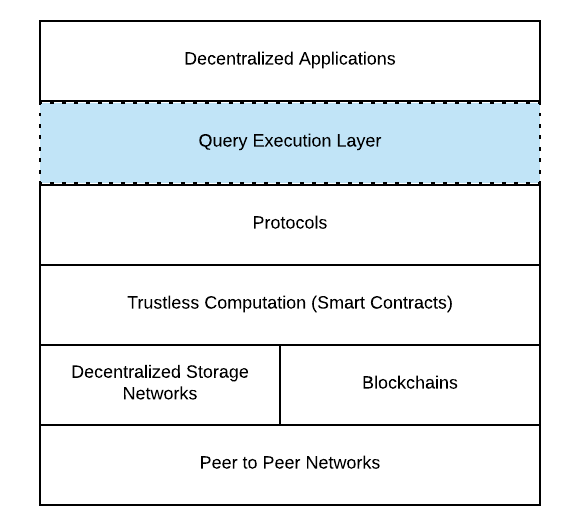
\includegraphics[width=0.6\textwidth]{media/image8.png}
\end{center}
\end{figure}
\noindent
An established decentralized \textit{Query Execution Layer} shown in Figure 1 does not currently exist. Without a decentralized Query Execution Layer for Web3, dApp developers must resort to building custom indexing servers on an ad-hoc basis. This introduces a centralized component and requires engineering and devops resources to build and maintain. Providing a decentralized Query Execution Layer would allow dApp developers to ship more reliable dApps faster with fewer resources. It would also enable dApps to become fully decentralized.
\subsection{Decentralized Query Protocol}
\subsubsection*{Definition}
A \textit{Decentralized Query Protocol} is defined to be a collection of rules by which clients pay a decentralized network of nodes for indexing, caching, and querying data that is stored on public blockchains and decentralized storage networks such as IPFS/Swarm.
\subsubsection*{Protocol Requirements}
In order to enable a new class of data-intensive dApps, a Decentralized Query Protocol must meet the following requirements:
\begin{enumerate}
\item \textit{Trust without verification}---a client should be able to trust the results of queries without independently verifying each query or loading the underlying raw data.
\item \textit{Metering}---a client should be able to efficiently pay for each query processed by the network, with minimal counterparty risk for either the client or the nodes.
\item \textit{Predictable performance}---the client should be able to pay for predictable performance for queries that are run against specific data sources.
\item \textit{Data availability---}a client should be able to pay to keep the data available for running queries against specific data sources.
\item \textit{Price efficiency}---clients should be able to pay for queries, performance, and data availability in efficient and competitive marketplaces.
\item \textit{Incentive alignment}---incentives should be aligned between clients, nodes, and dApp developers to encourage growth of the network and positive network effects.
\end{enumerate}
\section{Design}
The Graph implements a Decentralized Query Protocol, which enables users to query a network for data without having to operate any centralized infrastructure for indexing and caching. The protocol synthesizes ideas from distributed computing and cryptoeconomics\footnote{Vitalik Buterin, ``Introduction to Cryptoeconomics,'' Vitalik Buterin's Website, March 12, 2018,
https://vitalik.ca/files/intro\_cryptoeconomics.pdf} to produce a network that is self-organizing, robust, and secure.
\subsection{System Overview}
\subsubsection*{Protocol Stack}
The Graph can be divided into a stack of sub-protocols which can be treated conceptually as distinct interoperable layers, as shown in Figure 2.
\begin{figure}[H]
\vspace*{5mm}
\caption{\textbf{The Protocol Stack has the following sub-protocols:}}
\begin{center}
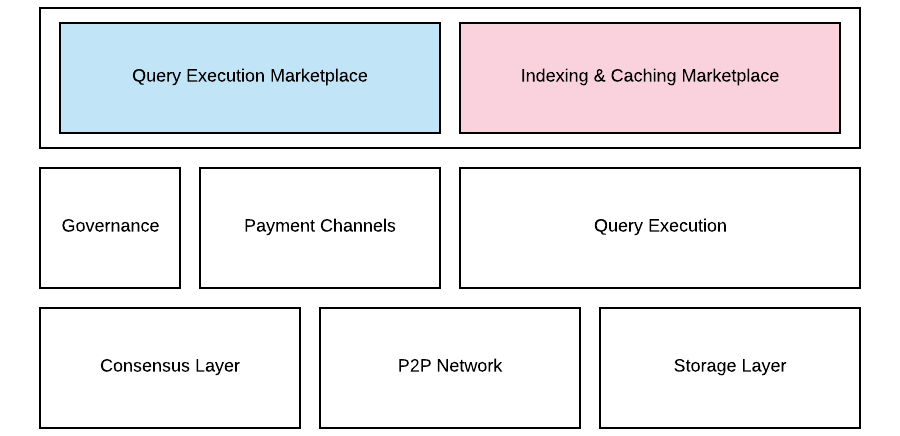
\includegraphics[width=.9\textwidth]{media/image7.png}
\end{center}
\end{figure}
\begin{enumerate}
\item \textbf{Consensus} \textbf{Layer---}responsible for smart contract execution and payment settlement.
\item \textbf{Peer-to-peer (P2P) Network}---defines how nodes locate and connect to each other.
\item \textbf{Storage Layer---}data stored on public blockchains or content addressable networks.
\item \textbf{Query Processing---}how a query is routed to a specific node for processing.
\item \textbf{Payment Channels---}facilitates fast and low-cost payments in the system.
\item \textbf{Governance---}manages schemas, data sources, and disputes.
\item \textbf{Query Marketplace}---mechanism by which users pay nodes for specific queries.
\item \textbf{Indexing and Caching Marketplace---}mechanism by which users pay nodes for indexing and caching data sources.
\end{enumerate}
\subsubsection*{Token}
The Graph introduces a new token, \textit{Graph Tokens}, which play a vital role in securing and governing the network. Each of the uses for the token will be described alongside their respective related sub-protocols and summarized in the Token Economics section of this document.
\subsubsection*{Query Language}
The Graph will support queries written in GraphQL, a query language invented and open-sourced by Facebook. While SQL might be more familiar to back-end engineers, it is not well-suited to running queries from front-end applications. Traditional web apps handle this impedance mismatch by writing centralized API servers and data access layers in front of SQL databases, which are then exposed as REST endpoints. Since a requirement of dApps is that they require no centralized infrastructure to function, it is important that dApp clients can query data directly from the front-end in a flexible way. GraphQL was designed to meet this criteria and has since seen accelerating adoption in the web and mobile communities.
\subsubsection*{Data Model}
All queries in The Graph are executed against a particular \textit{Data Source}. A Data Source is composed of a \textit{Schema} and one or more \textit{Datasets}.
\newline
\newline
The Schema is a GraphQL SDL schema, and defines the entities, values, types, and relationships which may be queried. Unlike in traditional databases, the Schema here is purely a logical definition, and doesn't dictate the structure of the data at the storage layer.
\newline
\newline
The Dataset defines data which exists on public blockchains or on decentralized storage networks that may be queried as part of a particular Data Source. It is composed of \textit{Data}\textbf{,} \textit{Mappings,} and an optional \textit{Update Function}.
\newline
\newline
Data identifies the raw data in the decentralized storage layer. It contains an identifier for the storage system being used, and the location of the raw data in that storage system. The location format will vary by storage system, for example a content hash on The InterPlanetary File System (IPFS) but a contract address on Ethereum.
The Mappings define how the Data maps to a particular Schema. It also includes metadata around the format in which the data is stored, such as CSV, Parquet, or a custom binary format.
\newline
\newline
The \textit{Update Function} is an optional script that can be provided for mutable data such as Ethereum contract data. It can also be provided for content-addressed data, which is referenced through a naming service such as IPNS rather than its content hash, which is immutable. The function accepts the data as input and returns an \textit{Update Event} which consists of a CUD (Create, Update, Delete) \textit{Operation} and a \textit{Payload}. The Update Event allows for performantly updating indexes without having to fully reindex the underlying Data.
\subsubsection*{Network Participants}
There are several types of participants in the network which are defined by their functional role in the protocol. With the exception of the dApp client, which is external to the protocol, a single node implementation may fulfill multiple functional roles.
\begin{enumerate}
\item \textit{dApp Client}---a front-end application running on the End User's machine which queries The Graph.
\item \textit{Gateway Node}\textbf{---}a node which acts as an HTTP, WebSocket, or JSON RPC endpoint for dApp clients to query The Graph.
\item \textit{P2P Node}\textbf{---}a node which participates in the P2P network.
\item \textit{Query Node}\textbf{---}a node which participates in query processing.
\end{enumerate}
\subsubsection*{Economic Agents}
There are several types of economic agents which we define by the common set of incentives that govern their usage of the protocol.
\begin{enumerate}
\item \textit{End User}\textbf{---}seeks to get utility from an application and pays to use the network.
\item \textit{dApp Developer}\textbf{---}seeks to monetize their work building a decentralized application for the End User.
\item \textit{Node Operator}\textbf{---}operates P2P Nodes and Query Nodes to extract fees and drive up the value of existing token holdings.
\item \textit{Data Source Curator}\textbf{---}creates and curates Data Sources in The Graph to extract interest and drive up the value of existing token holdings.
\item \textit{Validator}\textbf{---}validates query responses in exchange for interest and driving up the value of existing token holdings.
\end{enumerate}
\subsection{Sub-Protocols}
\subsubsection*{Consensus Layer}
The Graph has several components which require a blockchain-based consensus layer to provide guarantees that mechanisms in the protocol (payments, voting, validation, etc.) are immutable, irreversible, and can be carried out without the help of a central governing authority. We will use an existing blockchain such as Ethereum for this purpose.
\subsubsection*{Storage Integration Layer}
The Graph can support a variety of storage backends using Storage Adapters, an idea inspired by IPLD\footnote{``IPLD/specs,'' GitHub, accessed March 5, 2018. https://github.com/ipld/specs/tree/master/ipld.}. These may include Ethereum, IPFS, other blockchains, or other forms of decentralized storage.
\subsubsection*{P2P Network}
The Graph implements a structured overlay network which builds on ideas from \textit{Content-Addressable Networks (CANs}\textbf{\textit{)}} such as IPFS\footnote{Juan Benet, ``IPFS - Content Addressed, Versioned, P2P File System (DRAFT 3),'' IPFS, March 5, 2018,
https://ipfs.io/ipfs/QmR7GSQM93Cx5eAg6a6yRzNde1FQv7uL6X1o4k7zrJa3LX/ipfs.draft3.pdf} and BitTorrent\footnote{Andrew Lowenstern and Arvid Norberg, ``DHT Protocol,'' BitTorrent.org, May 1, 2017, http://www.bittorrent.org/beps/bep\_0005.html}. We introduce the concept of a \textit{Service-Addressable Network} to describe our formulation; the key difference is that while CANs leverage \textit{distributed hash tables (DHTs)} to locate nodes on the network storing a specific file or object\footnote{Sylvia Ratnasamy, P. Francis, M. Handley, R. Karp, and S. Shenker, ``A Scalable Content-Addressable Network,'' Proceedings of ACM SIGCOMM, August 2001, http://dx.doi.org/10.1145/383059.383072. }, our P2P network is used to locate nodes capable of providing a particular service, which can be any arbitrary computational work. The design of our P2P network sub-protocol is modular with respect to the service being provided, a fact which we take advantage of in other parts of the protocol stack.

\begin{figure}[H]
\vspace*{5mm}
\caption{\textbf{Service-Addressable Network}}
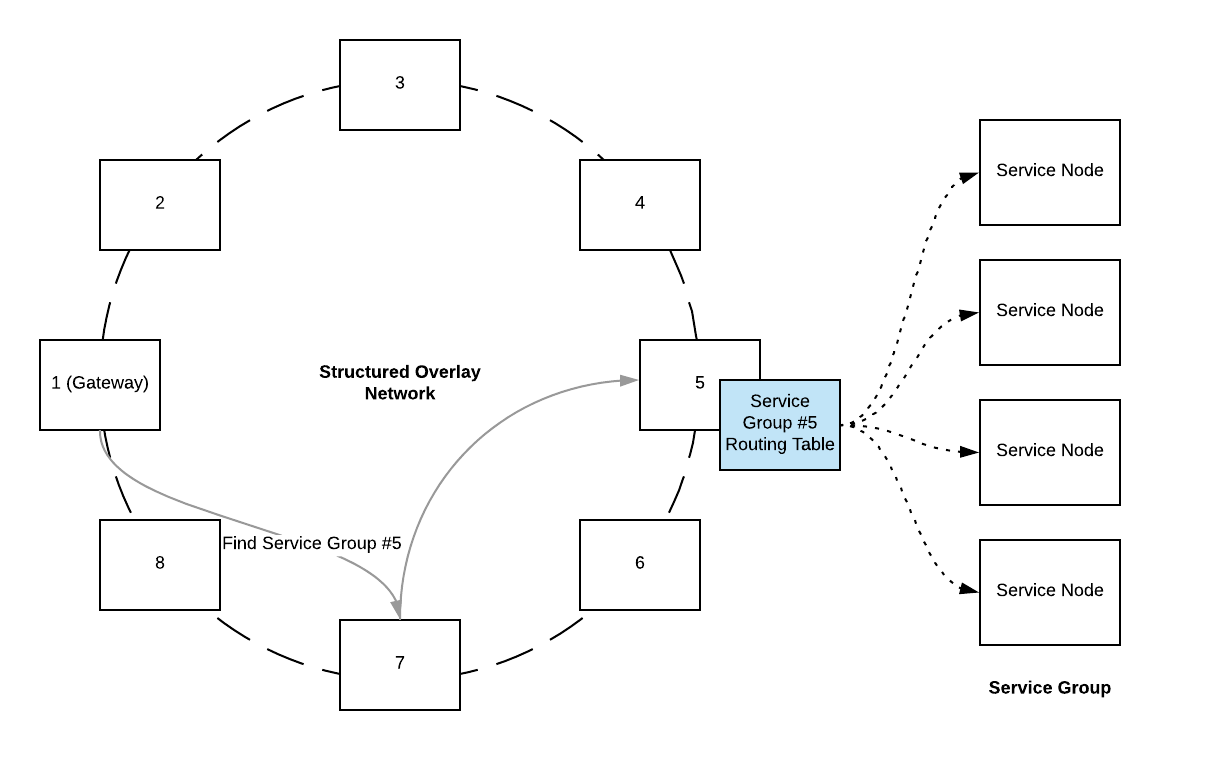
\includegraphics[width=1\textwidth]{media/image6.png}
\end{figure}
\subsubsection*{Query Processing}
The \textit{Query Processing} is split into five distinct stages: \textit{Query Splitting, Service Discovery, Query Routing, Nested Query Processing} and \textit{Response Collation}.
\subsubsection*{Query Splitting}
The first step of the Query Processing sub-protocol is to split a query into disjoint top-level \textit{Query Fragments,} which may correspond to multiple Data Sources. A Query Fragment is any part of a query that can be resolved on its own. These fragments are processed separately, moving through the subsequent Query Processing stages in parallel.
\subsubsection*{Service Discovery}
In the Service Discovery stage, we leverage our Service-Addressable Network, to locate a P2P Node, with a routing table corresponding to a specific Service Group, as shown in Figure 4. In the context of this sub-protocol we define the Service Group to be a group of Query Nodes capable of processing a query for a specific Data Source.
\begin{figure}[H]
\caption{\textbf{The Service Discovery stage.}}
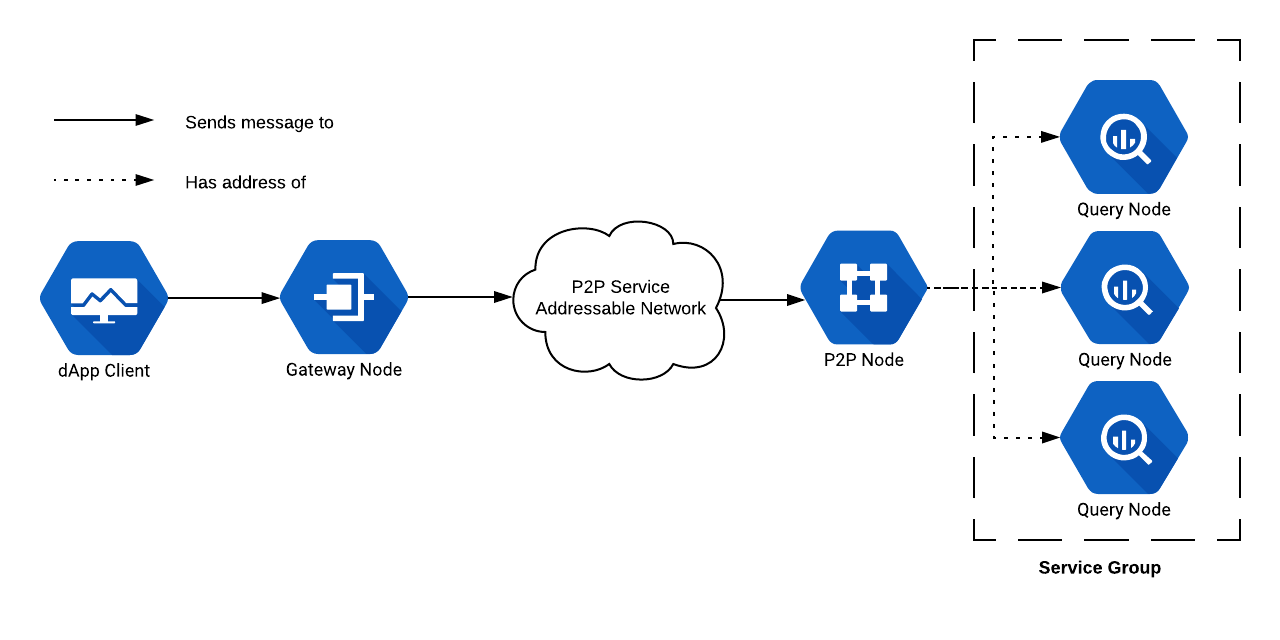
\includegraphics[width=1\textwidth]{media/image10.png}
\end{figure}
\subsubsection*{Query Routing}
In the Query Routing stage, the Gateway Node that originated the query\footnote{From the perspective of the network, it is impossible to distinguish whether a Gateway Node originated a query itself, or on behalf of a dApp client.} decides which Query Node to forward a specific Query Fragment to, as shown in Figure 5. The Query Routing stage uses the \textit{Service Group Routing Table}, which contains the location of each Node in the Service Group, as well as additional metadata.
\begin{figure}[H]
\caption{\textbf{The Query Routing stage.}}
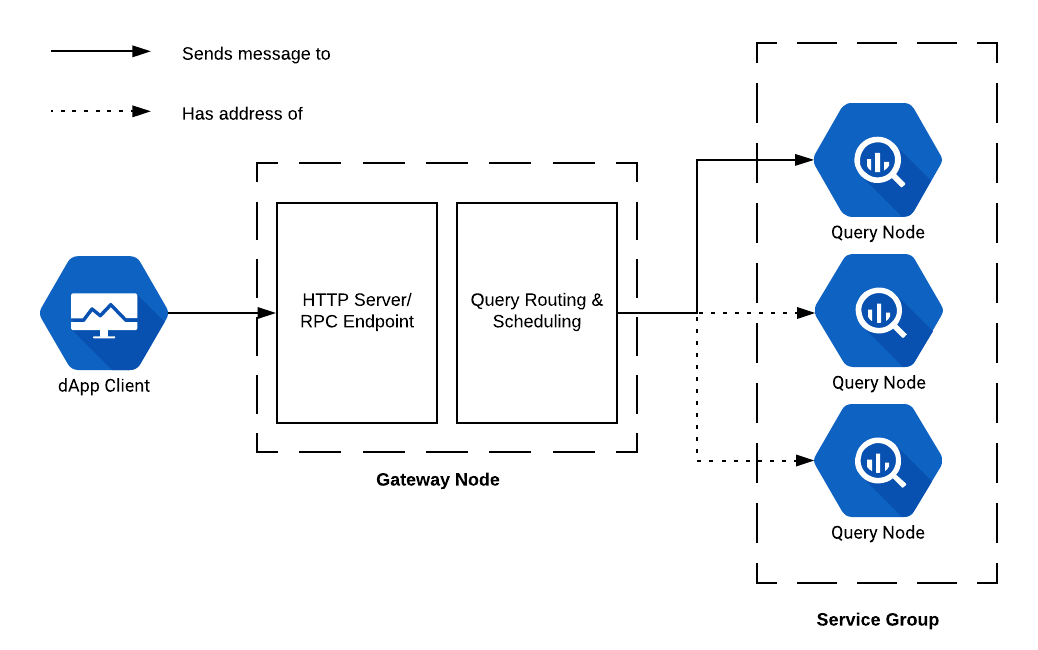
\includegraphics[width=1\textwidth]{media/image9.png}
\end{figure}
\noindent
The metadata in the Service Group Routing Table is extensible to support modular routing logic. We take advantage of this in the Query Marketplace sub-protocol, but it could also be used to support operating the protocol in local networks or with trusted nodes, where payment requirements may be undesirable.
\subsubsection*{Nested Query Processing}
Each Query Fragment corresponds to a single entity type that is indexed by The Graph. If the user wishes to traverse nested entity relationships, these are processed as separate Query Fragments which go through the steps listed above. Queries may be arbitrarily deep, and thus are processed recursively, in serial until all the Query Fragments are processed.
\subsubsection*{Response Collation}
The final stage is to await execution of all the Query Fragments, both in series and in parallel, and to collate the responses in a format that meets the GraphQL specification\footnote{http://facebook.github.io/graphql/draft/} for the given query.
\subsubsection*{Payment Channels}
In order to keep throughput high and transaction cost low, the network will use \textit{Payment Channels} for microtransactions\footnote{https://lightning.network/lightning-network-paper.pdf}. Payment Channels may be opened directly between two nodes, but for the flexibility of the protocol, it is appropriate to use a network of Payment Channels such as Raiden\footnote{https://raiden.network/}, which allows for payments to be made between many-to-many nodes without having to settle on-chain for each new node-to-node transaction. In this way, a single Payment Channel could be opened once by an End User to support many microtransactions for metered usage of The Graph. The Payment Channels could then be settled on-chain on a desired cadence.
\subsubsection*{Governance}
Since The Graph provides the main API endpoint for dApps to query data, deciding what data to include in query results impacts users and developers. The Graph provides a way for the community to vote and decide on what data to include and exclude. For example there may be competing protocols for any given domain. The network could choose to include data from one protocol or multiple.
\newline
\newline
To start using The Graph, a dApp developer needs to make sure that a Schema exists for their domain. A Schema is composed of namespaces, entities, fields, and relationships between entities. If entities or fields are missing from the global Schema, a developer can propose changes by staking tokens. Schema changes can only be accretive and cannot include breaking changes to ensure that deployed dApps do not break.
\newline
\newline
Once a Schema exists for a domain, a dApp developer can propose to include a new Data Source for an entity by staking tokens. Other developers working in the same domain will want to check to make sure that the Data Source is high quality and compatible since new Data Sources would have an impact on their dApps. If quality Data Sources are added, their dApps will work better and their users will be happy. If the new Data Source produces spam or low quality content, developers will have an incentive to reject it. Participation in the governance process through staking will be rewarded with token inflation based on how much value the Data Sources drive to the network.
\subsubsection*{Query Marketplace}
The Query Marketplace lets End Users pay Query Nodes for individual queries (or Query Fragments) issued against a specific Data Source. The Query Marketplace builds on top of the extensible P2P Network and Query Routing sub-protocols. We leverage the extensible Service Group Routing Table metadata to list a \textit{Price Sheet} which Query Nodes may use to advertise the fees they will charge to process queries for a specific Data Source. The fees will be priced in terms of estimated complexity of the query, size of the query response, and latency. We route the query to a specific Query Node to achieve the desired tradeoff of cost and performance for any given query. The Gateway Node may optionally expose this logic in its query interface such that dApp developers or End Users may specify the optimal cost versus performance tradeoff for their specific use case.
\newline
\newline
Query Nodes must bond a desired number of Graph Tokens in order to participate in the marketplace. The more tokens they bond, the more likely they are to be seen as trustworthy by users of the network and be able to extract fees for queries. While most transactions of payment for query processing will occur off-chain, an End User or Gateway Node may challenge any specific query response by creating a \textit{Dispute} on-chain, which is a voting smart contract in which a set of Validators votes on the correctness of a query response in a commit and reveal process. If the challenge succeeds, then the Query Node's bonded tokens are forfeited to the challenger who created the Dispute. Validator Nodes are rewarded for securing the marketplace through token inflation.
\subsubsection*{Indexing and Caching Marketplace}
While the Query Marketplace incentivizes Query Nodes to respond to individual queries, it does not provide any guarantees that there are Query Nodes which are available to process the query performantly. This can be problematic, especially when bootstrapping a new Data Source which does not yet have usage. The Indexing and Caching marketplace allows Query Nodes to be compensated for providing a specific \textit{Service-level Agreement} \textbf{\textit{(}}\textit{SLA}\textbf{\textit{)}} which is a promise to be available to process queries for a specific Data Source within certain latency and cost bounds. If a Query Node is found to be in violation of the SLA then its staked tokens will be forfeited to the user who paid for the SLA. The network may implement a challenge-response protocol to verify that an SLA is being met even when users are not actively querying that Data Source.
\section{Token Economics}
Graph Tokens are used to secure and govern the network and to incentivize behaviors that are critical for the network to thrive. Token mechanics are described in relevant sections of the protocol, but we provide here a consolidated list of the mechanisms that involve tokens, and how specific economic agents interact with the tokens. Graph Tokens:
\begin{itemize}
\item Are bonded by Query Nodes to participate in the Query Marketplace as well as the Indexing and Caching Marketplace.
\item Are bonded by Validators to participate in voting in on-chain Disputes.
\item Are staked by Challengers to create a Dispute.
\item Are paid to Validators through token inflation.
\item Are paid to Data Source curators through token inflation.
\item Are used in decentralized governance mechanisms for a specific Data Source (i.e. Token Curated Registries).
\item May be used as fees in the Query Marketplace as well as the Indexing and Caching Marketplace
\end{itemize}
\section{Roadmap}
Our plan is to release The Graph across three major development milestones. The first release will be a free service that any dApp developer can register to use. It will include stable interfaces for defining the Schema, registering Mappings, and querying with GraphQL. This release is slated for Q3 2018. Launching first as a centralized service will allow us to iterate on the design, implementation, and economic incentives at a faster rate. The second milestone will be the launch of the full P2P network in 2019. After this release, anyone will be able to run a Graph Node and earn Graph Tokens for participating in the network. This is the stage at which the Query Marketplace as well as the Indexing and Caching Marketplace will be opened. The third major release will include support for Private Data. Private Data is anchored on-chain but encrypted and controlled by users. This release is scheduled for 2020.
\section{Conclusion}
In this paper we presented the requirements for a Decentralized Query Protocol\textit{,} a set of rules by which clients pay a decentralized network of nodes for indexing, caching, and querying data that is stored on public blockchains and decentralized storage networks. We provided a high-level overview of The Graph, our formulation of a Decentralized Query Protocol. We also proposed our definition for what constitutes a dApp---a dApp must put users in control of their data. dApps are built using data that is either owned and managed by the community or is private and controlled by the user. This way many products and services can be built on interchangeable Datasets and users can freely switch between dApps. The Graph acts as an interoperability layer that will enable these flourishing ecosystems of interoperable dApps to thrive and replace centrally controlled data monopolies.
\end{document}
